\documentclass{standalone}
\usepackage[svgnames]{xcolor}
\usepackage{tikz}

%LIBRERIAS	
	\usetikzlibrary{decorations.markings}
	\usetikzlibrary{shapes.geometric}
	\usetikzlibrary{arrows}
	\usetikzlibrary{shapes.symbols}

%LAYERS
	\pgfdeclarelayer{leyenda}
	\pgfdeclarelayer{lineas_layer}
	\pgfdeclarelayer{esquema}
	\pgfsetlayers{lineas_layer,esquema,leyenda,main}

%ESTILOS
	\tikzstyle{none}=[inner sep=0pt]
	\tikzstyle{tratamientos}=[draw=Orange,fill=white,font=\fontsize{7}{7}\selectfont,inner sep=2pt]
	\tikzstyle{tratamientos2}=[draw=Orange,fill=white,font=\fontsize{7}{7}\selectfont,inner sep=2pt,text width=2cm,align=center]
	\tikzstyle{tratamientos3}=[draw=Orange,fill=white,font=\fontsize{7}{7}\selectfont,inner sep=2pt,align=left,anchor=west]
	\tikzstyle{estrella}=[starburst, draw,,font=\fontsize{7}{7}\selectfont, text width=2cm,red,fill=orange,line width=1pt,align=center]
	\tikzstyle{caract}=[draw=Gray,fill=Gray,font=\fontsize{7}{7}\selectfont,align=center,inner sep=2pt,text width=4cm]
	\tikzstyle{sustrato}=[circle,fill=Red!60,draw=Black,line width=0.8 pt]
	\tikzstyle{poros}=[circle,fill=Orange,draw=Black,line width=0.8 pt]
	\tikzstyle{sol}=[circle,text width=1.8cm,align=center,fill=Yellow,draw=Black,line width=0.8 pt]
	\tikzstyle{line} = [draw,-latex']
	\tikzstyle{simple}=[-latex',draw=darkgray,line width=0.5]
	% \tikzstyle{lateral}=[<-,draw=darkgray,line width=0.5]
	% \tikzstyle{lateral2}=[->,draw=darkgray,line width=0.5]
	% \tikzstyle{corto}=[->,draw=red,line width=0.5,shorten >=0.5cm,shorten <=0.5cm]
	% \tikzstyle{corto_arriba}=[-,draw=red,line width=0.5,shorten <=0.3cm]
	% \tikzstyle{corto_abajo}=[-,draw=red,line width=0.5,shorten >=0.3cm]
	\tikzstyle{arrow}=[-,draw=Black,postaction={decorate},decoration={markings,mark=at position .5 with {\arrow{>}}},line width=2.000]
	\tikzstyle{tick}=[-,draw=Black,postaction={decorate},decoration={markings,mark=at position .5 with {\draw (0,-0.1) -- (0,0.1);}},line width=2.000]

\begin{document}
\begin{tikzpicture}
	
%%% SOL y POROS
 \begin{pgfonlayer}{esquema}
	\node [style=sol] (sol) at (0, 12) {solucion precursores};
	\node [style=poros] (ctab) at (-5, 9.5) {CTAB};
	\node [style=poros] (f127) at (5, 9.5) {F127};
	\node [style=tratamientos2] (deposito_ctab) at (-5, 8) {Deposito de PDM};
	\node [style=tratamientos2] (deposito_f127) at (5, 8) {Deposito de PDM};
	\node [style=sustrato] (Vi) at (-8, 6) {Vidrio};
	\node [style=sustrato] (Si) at (-5, 6) {Silicio};
	\node [style=sustrato] (Au) at (-3, 6) {Electrodos};
 \end{pgfonlayer}

% LINEAS SOL y POROS
 \begin{pgfonlayer}{lineas_layer}
	 \path [style=line] (sol) -- node {}(ctab);
		 \path [style=line] (ctab) -- node {}(deposito_ctab);
		 \path [style=line] (deposito_ctab) -- node {}(Vi);
		 \path [style=line] (deposito_ctab) -- node {}(Si);
		 \path [style=line] (deposito_ctab) -- node {}(Au);
	 \path [style=line] (sol) -- node {}(f127);
	 \path [style=line] (f127) -- node {}(deposito_f127);
 \end{pgfonlayer}
		 
%%% TRATAMIENTOS CTAB %%%%%%
		\node [style=none]	(tratamientos) at (-6.5,1.68) {
		\begin{tikzpicture}
		\begin{pgfonlayer}{esquema}
			\node [style=none] (Vi_virtual) at (-8,1) {};
			\node [style=none] (Si_virtual) at (-5,1) {};
			\node [style=tratamientos] (calcinado) at (-8, -3.75) {Calcinado};
			\node [style=tratamientos] (calcinado2) at (-5, -3.75) {Calcinado};
			\node [style=tratamientos] (simplificado) at (-6.9, -0) {Simplificado};
			\node [style=tratamientos] (prolongado) at (-6.55, -0.75) {Prolongado};
			\node [style=tratamientos] (acido) at (-6.5, -1.4) {Acido};
			\node [style=tratamientos] (basico) at (-6, -2.15) {Basico};
			\node [style=tratamientos] (vacio) at (-5.7, -3) {Vacio};
			\node [style=tratamientos] (extraccion) at (-6.5, -4.5) {Extraccion};
			\node [style=caract] (caract) at (-6.5, -6) {Multiples Caracterizaciones\\(SEM, FTIR, EPA)\\No apto para EQ};
		\end{pgfonlayer}
		\begin{pgfonlayer}{lineas_layer}
			 \path [style=line] (Vi_virtual) -- node {}(calcinado);
			 \path [style=line] (Vi_virtual) |- node {}(simplificado);
			 \path [style=line] (Vi_virtual) |- node {}(prolongado);
			 \path [style=line] (Vi_virtual) |- node {}(acido);
			 \path [style=line] (Vi_virtual) |- node {}(basico);
			 \path [style=line] (Vi_virtual) |- node {}(vacio);
			 \path [style=line] (Si_virtual) -- node {}(calcinado2);
			 \path [style=line] (Si_virtual) |- node {}(simplificado);
			 \path [style=line] (Si_virtual) |- node {}(prolongado);
			 \path [style=line] (Si_virtual) |- node {}(acido);
			 \path [style=line] (Si_virtual) |- node {}(basico);
			 \path [style=line] (Si_virtual) |- node {}(vacio);
			 \path [style=none,-latex'] ([xshift=1mm]simplificado.west) edge[in=120,out=270] (extraccion);
			 \path [style=none,-latex'] ([xshift=1mm]prolongado.west) edge[in=110,out=270] (extraccion);
			 \path [style=none,-latex'] ([xshift=1mm]acido.west) edge[in=90,out=270] node {}(extraccion);
			 \path [style=none,-latex'] ([xshift=1mm]basico.west) edge[in=80,out=270] node {}(extraccion);
			 \path [style=none,-latex'] ([xshift=1mm]vacio.west) edge[in=70,out=270] node {}(extraccion);
			 \path [style=none,-latex'] (calcinado.center) edge[transform canvas={xshift=-2mm},in=120,out=270] node {}(caract);
			 \path [style=none,-latex'] (calcinado2.center) edge[transform canvas={xshift=2mm},in=70,out=270] node {}(caract);
			 \path [style=line] (extraccion.center) -- node {}(caract);
		\end{pgfonlayer}
		\end{tikzpicture}
		};

%%%%  Superficie Modificada 
	\begin{pgfonlayer}{esquema}
		\node [style=tratamientos2] (sup) at (-2, 8) {Modificacion superficial};
	\end{pgfonlayer}
	\begin{pgfonlayer}{lineas_layer}
		\path [style=none,-latex'] (sup.west) edge[in=130,out=180] node {}(Au);
	\end{pgfonlayer}

%%% TRATAMIENTOS AU CTAB %%%%%%
		\node [style=none]	(tratamientos) at (-0.95,1.73) {
		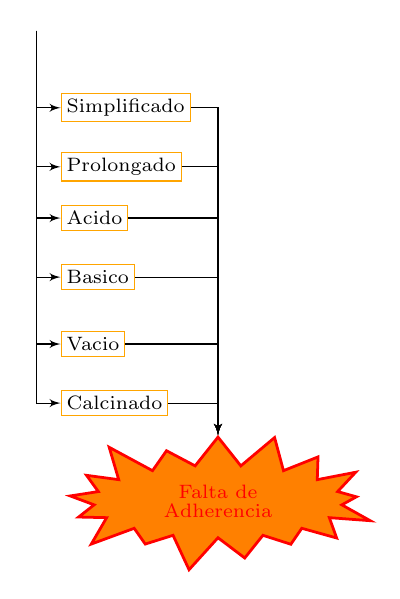
\begin{tikzpicture}
		\begin{pgfonlayer}{esquema}
			\node [style=none] (Au_virtual) at (-8.3,1) {};
			\node [style=tratamientos3] (calcinado) at (-8, -3.75) {Calcinado};
			\node [style=tratamientos3] (simplificado) at (-8, -0) {Simplificado};
			\node [style=tratamientos3] (prolongado) at (-8, -0.75) {Prolongado};
			\node [style=tratamientos3] (acido) at (-8, -1.4) {Acido};
			\node [style=tratamientos3] (basico) at (-8, -2.15) {Basico};
			\node [style=tratamientos3] (vacio) at (-8, -3) {Vacio};
			\node [style=estrella] (adherencia) at (-6,-5) {Falta de Adherencia};
    	\end{pgfonlayer}
		\begin{pgfonlayer}{lineas_layer}
   			 \path [style=line] (Au_virtual) |- node {}(simplificado);
			 \path [style=line] (Au_virtual) |- node {}(prolongado);
			 \path [style=line] (Au_virtual) |- node {}(acido);
			 \path [style=line] (Au_virtual) |- node {}(basico);
			 \path [style=line] (Au_virtual) |- node {}(vacio);
			 \path [style=line] (Au_virtual) |- node {}(calcinado);
			 \path [style=line] (calcinado) -| node {}(adherencia);
			 \path [style=line] (simplificado) -| node {}(adherencia);
			 \path [style=line] (prolongado) -| node {}(adherencia);
			 \path [style=line] (acido) -| node {}(adherencia);
			 \path [style=line] (basico) -| node {}(adherencia);
			 \path [style=line] (vacio) -| node {}(adherencia);
		\end{pgfonlayer}
		\end{tikzpicture}
		};

%%% TRATAMIENTOS F127 (Si / Vi) %%%%%%
		\node [style=none]	(tratamientos) at (-6.5,1.68) {
		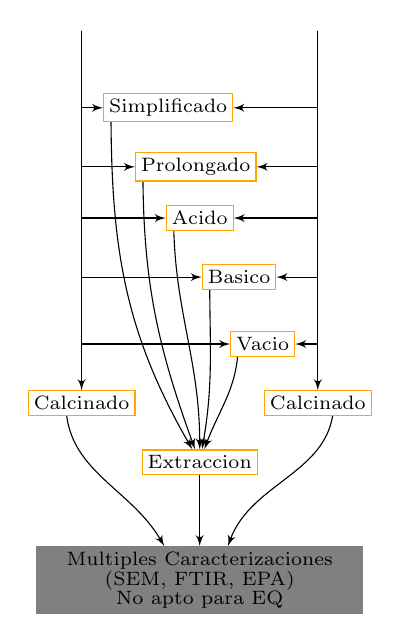
\begin{tikzpicture}
		\begin{pgfonlayer}{esquema}
			\node [style=none] (Vi_virtual) at (-8,1) {};
			\node [style=none] (Si_virtual) at (-5,1) {};
			\node [style=tratamientos] (calcinado) at (-8, -3.75) {Calcinado};
			\node [style=tratamientos] (calcinado2) at (-5, -3.75) {Calcinado};
			\node [style=tratamientos] (simplificado) at (-6.9, -0) {Simplificado};
			\node [style=tratamientos] (prolongado) at (-6.55, -0.75) {Prolongado};
			\node [style=tratamientos] (acido) at (-6.5, -1.4) {Acido};
			\node [style=tratamientos] (basico) at (-6, -2.15) {Basico};
			\node [style=tratamientos] (vacio) at (-5.7, -3) {Vacio};
			\node [style=tratamientos] (extraccion) at (-6.5, -4.5) {Extraccion};
			\node [style=caract] (caract) at (-6.5, -6) {Multiples Caracterizaciones\\(SEM, FTIR, EPA)\\No apto para EQ};
		\end{pgfonlayer}
		\begin{pgfonlayer}{lineas_layer}
			 \path [style=line] (Vi_virtual) -- node {}(calcinado);
			 \path [style=line] (Vi_virtual) |- node {}(simplificado);
			 \path [style=line] (Vi_virtual) |- node {}(prolongado);
			 \path [style=line] (Vi_virtual) |- node {}(acido);
			 \path [style=line] (Vi_virtual) |- node {}(basico);
			 \path [style=line] (Vi_virtual) |- node {}(vacio);
			 \path [style=line] (Si_virtual) -- node {}(calcinado2);
			 \path [style=line] (Si_virtual) |- node {}(simplificado);
			 \path [style=line] (Si_virtual) |- node {}(prolongado);
			 \path [style=line] (Si_virtual) |- node {}(acido);
			 \path [style=line] (Si_virtual) |- node {}(basico);
			 \path [style=line] (Si_virtual) |- node {}(vacio);
			 \path [style=none,-latex'] ([xshift=1mm]simplificado.west) edge[in=120,out=270] (extraccion);
			 \path [style=none,-latex'] ([xshift=1mm]prolongado.west) edge[in=110,out=270] (extraccion);
			 \path [style=none,-latex'] ([xshift=1mm]acido.west) edge[in=90,out=270] node {}(extraccion);
			 \path [style=none,-latex'] ([xshift=1mm]basico.west) edge[in=80,out=270] node {}(extraccion);
			 \path [style=none,-latex'] ([xshift=1mm]vacio.west) edge[in=70,out=270] node {}(extraccion);
			 \path [style=none,-latex'] (calcinado.center) edge[transform canvas={xshift=-2mm},in=120,out=270] node {}(caract);
			 \path [style=none,-latex'] (calcinado2.center) edge[transform canvas={xshift=2mm},in=70,out=270] node {}(caract);
			 \path [style=line] (extraccion.center) -- node {}(caract);
		\end{pgfonlayer}
		\end{tikzpicture}
		};

\end{tikzpicture}

\end{document}